\section{SEM}

% ~5 Bilder
% tif-Dateien: je 2 Bilder, eins bse, eins se
% Vergrößerung im Bild ist manchmal falsch. auf die im Dateinahmen achten. aber die scale bar ist eh ausreichend
% what have we seen: charging artefacts (bad sample coating/high magnification, charge buildup)
%bse/se difference (bse gives composition: heavy elements),
%piece of insect antenna: auflösungslimit, astigmatismuskorrektu wird während Bildaufnahme geändert=>Streifen im Bild
%Insektenaugen: rechts implodiert, links nicht



In \cref{fig:insekt_implosion} ist die Sekundärelektronenaufnahme eines Insektenkopfs bei unterschiedlichen Vergrößerungen dargestellt.
Es ist deutlich zu erkennen, dass hier eine erhebliche Beschädigung des Probenobjekts durch den Trocknungsprozess vorliegt.
Dadurch, dass das Insekt an Atmosphärenluft getrocknet ist, sind die Facetten der Augen implodiert.
Zum Vergleich ist in \cref{fig:mottenauge} die Aufnahme eines Mottenauges abgebildet, bei dem eine solche Implosion trotz Lufttrocknung nicht vorliegt.



\begin{figure}[!ht]
    \centering
    \begin{subfigure}{0.465\textwidth}
        \centering
        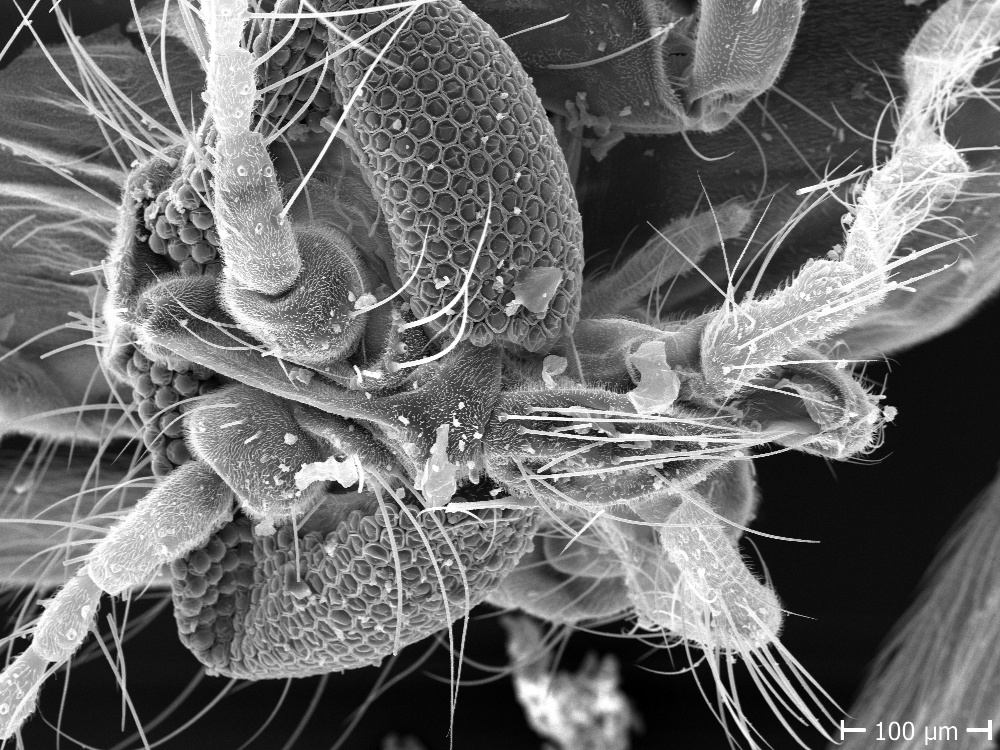
\includegraphics[width=1.1\textwidth]{img/SEM/10.9.20 9_08_08_Mag_ 180x_SE_insect_.jpg}
    \caption{}
    \end{subfigure}
    \hfill
    \begin{subfigure}{0.465\textwidth}
        \centering
        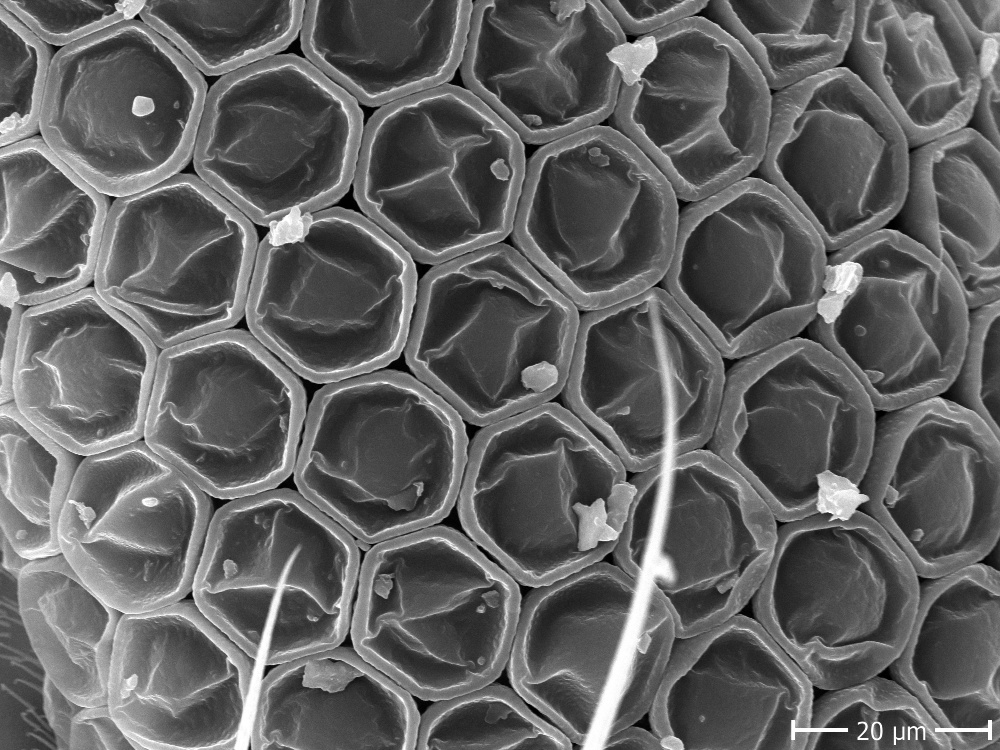
\includegraphics[width=1.1\textwidth]{img/SEM/10.9.20 9_11_43_Mag_ 1200x_SE_insect_eye_drying_artififact.jpg}
        \caption{}
    \end{subfigure}
    \caption{Sekundärelektronenaufnahmen eines luftgetrockneten Insektenkopfs bei unterschiedlichen Vergrößerungen.}
      \label{fig:insekt_implosion}
\end{figure}

\begin{figure}[!ht]
    \centering
    \begin{subfigure}{0.465\textwidth}
        \centering
        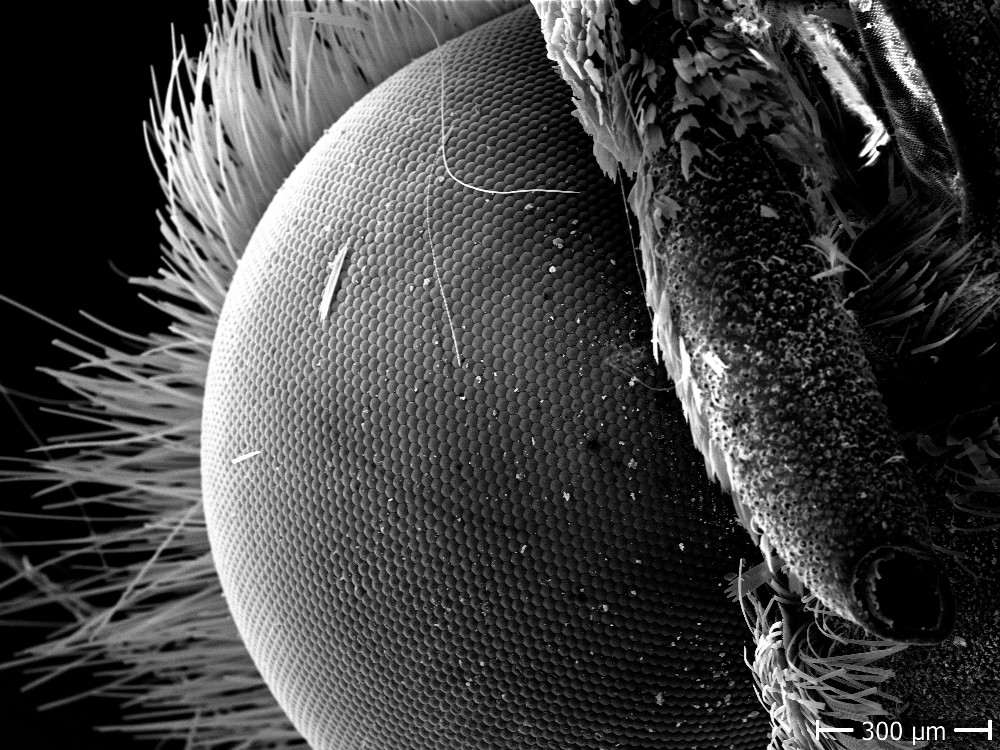
\includegraphics[width=1.1\textwidth]{img/SEM/10.9.20 9_44_08_Mag_ 70x_SE_moth_eye}
    \caption{}
    \end{subfigure}
    \hfill
    \begin{subfigure}{0.465\textwidth}
        \centering
        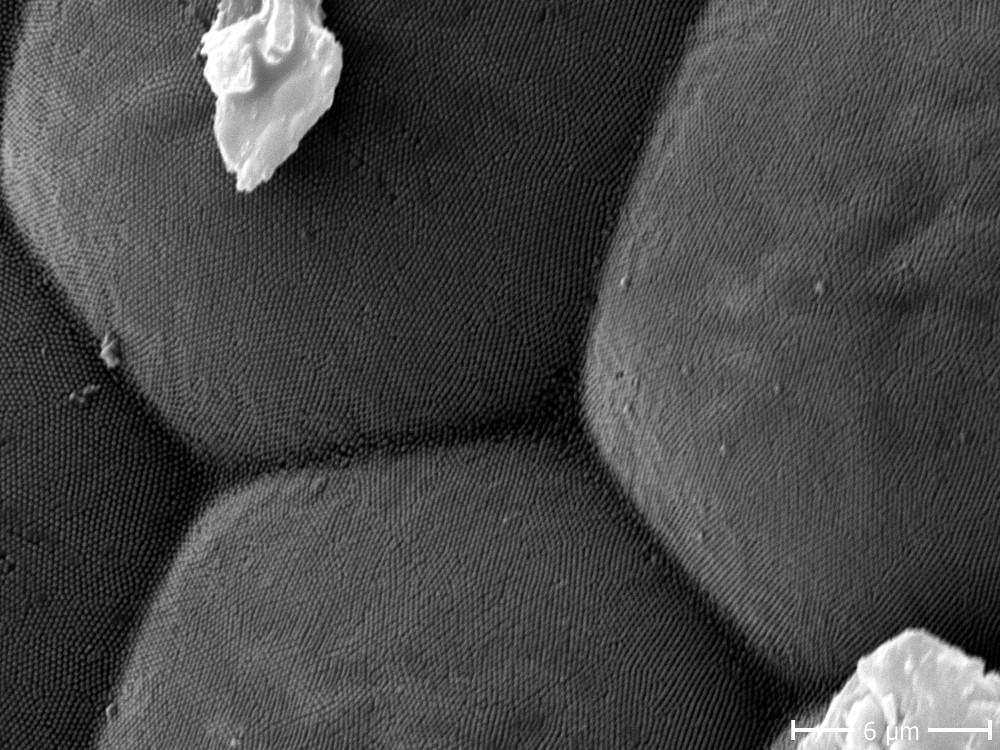
\includegraphics[width=1.1\textwidth]{img/SEM/10.9.20 9_46_35_Mag_ 4000x_SE_moth_eye}
        \caption{}
    \end{subfigure}
    \caption{Sekundärelektronenaufnahmen eines luftgetrockneten Mottenauges bei unterschiedlichen Vergrößerungen.}
      \label{fig:mottenauge}
\end{figure}

In der Aufnahme einer Insektenantenne in \cref{fig:astigmatenne} wurde während des Scans die Astigmatismuskorrektur geändert.
Dies drückt sich im Bild anhand von horizontalen Streifen aus.

\begin{figure}[!ht]
    \centering
    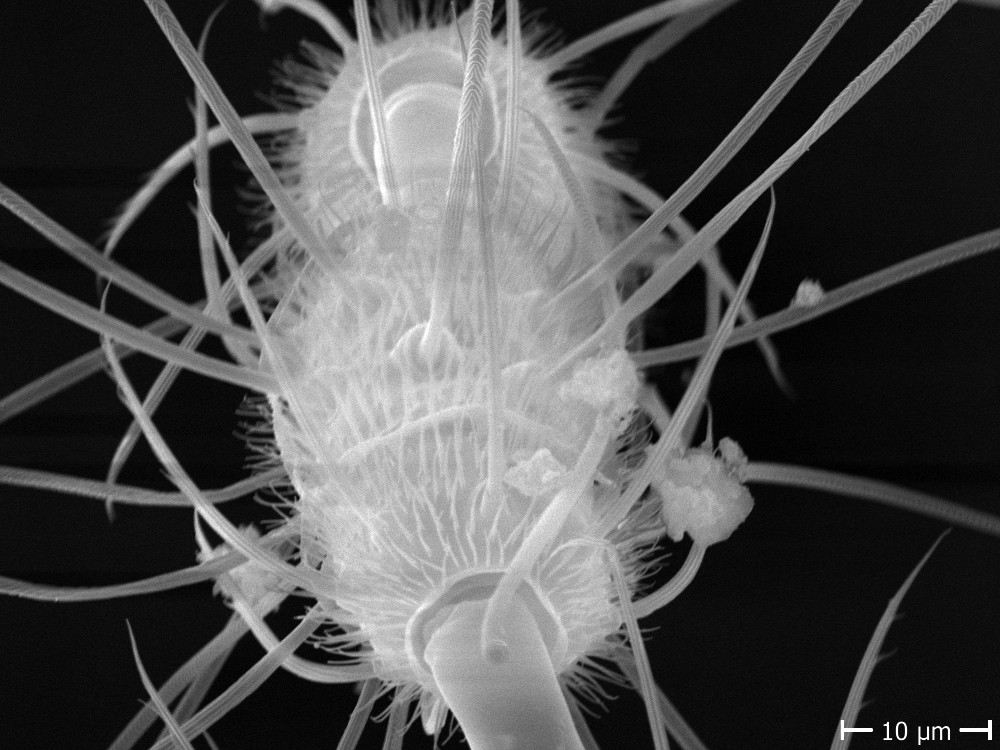
\includegraphics[width=0.65\textwidth]{img/SEM/10.9.20 11_09_41_Mag_ 1800x_astigmatism_introduced}
    \caption{Sekundärelektronenaufnahme der Antenne eines Insekts. Während der Aufnahme wurde die Astigmatismuskorrektur geändert.}
    \label{fig:astigmatenne}
\end{figure}
